%  article.tex (Version 3.3, released 19 January 2008)
%  Article to demonstrate format for SPIE Proceedings
%  Special instructions are included in this file after the
%  symbol %>>>>
%  Numerous commands are commented out, but included to show how
%  to effect various options, e.g., to print page numbers, etc.
%  This LaTeX source file is composed for LaTeX2e.

%  The following commands have been added in the SPIE class 
%  file (spie.cls) and will not be understood in other classes:
%  \supit{}, \authorinfo{}, \skiplinehalf, \keywords{}
%  The bibliography style file is called spiebib.bst, 
%  which replaces the standard style unstr.bst.  

\documentclass[A4]{spie}  %>>> use for US letter paper
%%\documentclass[a4paper]{spie}  %>>> use this instead for A4 paper
%%\documentclass[nocompress]{spie}  %>>> to avoid compression of citations
%% \addtolength{\voffset}{9mm}   %>>> moves text field down
%% \renewcommand{\baselinestretch}{1.65}   %>>> 1.65 for double spacing, 1.25 for 1.5 spacing 
%  The following command loads a graphics package to include images 
%  in the document. It may be necessary to specify a DVI driver option,
%  e.g., [dvips], but that may be inappropriate for some LaTeX 
%  installations. 
\usepackage[]{graphicx}

\title{Absolute calibration of gravitational wave detector using gravity field and photon pressure} 

%>>>> The author is responsible for formatting the 
%  author list and their institutions.  Use  \skiplinehalf 
%  to separate author list from addresses and between each address.
%  The correspondence between each author and his/her address
%  can be indicated with a superscript in italics, 
%  which is easily obtained with \supit{}.

\author{Yuki Inoue\supit{a,b}, Sadakazu Haino\supit{a}, Nobuyuki Kanda\supit{c}, Yujiro Ogawa\supit{b}, Toshikazu Suzuki,\supit{d}, Takayuki Tomaru\supit{b}, Takahiro Yamamoto\supit{e}, Takaaki Yokozawa\supit{e}
\skiplinehalf
\supit{a}Institute of Physics, Academia Sinica, Nankang, Taipei 11529, Taiwan; \\
\supit{b}High Energy Accelerator Research Organization, Tsukuba, Ibaraki, 305-0801, Japan;\\
\supit{c}Department of Physics, Osaka City University, Sumiyoshi, Osaka 558-8585, Japan;\\
\supit{d}Institute for Cosmic Ray Research, University of Tokyo, Kashiwa, Chiba, 277-8582, Japan;\\
\supit{e}KAGRA Observatory, Institute for Cosmic Ray Research, University of Tokyo, Hida, Gifu 506-1205, Japan;\\
}

%>>>> Further information about the authors, other than their 
%  institution and addresses, should be included as a footnote, 
%  which is facilitated by the \authorinfo{} command.

\authorinfo{Yuki Inoue: iyuki@post.kek.jp}
%%>>>> when using amstex, you need to use @@ instead of @
 

%%%%%%%%%%%%%%%%%%%%%%%%%%%%%%%%%%%%%%%%%%%%%%%%%%%%%%%%%%%%% 
%>>>> uncomment following for page numbers
% \pagestyle{plain}    
%>>>> uncomment following to start page numbering at 301 
%\setcounter{page}{301} 
 
  \begin{document} 
  \maketitle 

%%%%%%%%%%%%%%%%%%%%%%%%%%%%%%%%%%%%%%%%%%%%%%%%%%%%%%%%%%%%% 
\begin{abstract}
Absolute calibration of the gravitational wave detectors are an essential to understand the source parameters of the gravitational wave source. The photon calibrator is primary calibrator and can calibrate the absolute displacement of the mirror by using the photon pressure.Current limit of the uncertainty of the absolute laser calibration is 3 \% corresponding to the absolute laser power of the photon calibrator.  In order to reduce the uncertainty of the photon calibrator, we propose a use of the gravity field calibrator. The gravity field calibrator can be modulated the mirror using the gravity gradient. To cancel the uncertainty of the distance between mirror and calibrator, we employed the quadrupole and hexapole mass distribution in the gravity field calibrator. This method can be estimated as the distance with ratio of the quadruple and hexapole response. We also estimated the systematic error of the geometry of the calibrator, transfer function and higher order effect of the multipole moment. The estimated precision of absolute calibration is 0.XXX\%, which is 10 times less than that of previous method.

\end{abstract}

%>>>> Include a list of keywords after the abstract 

\keywords{Gravitational Wave, KAGRA, LIGO, Virgo, Calibration}

%%%%%%%%%%%%%%%%%%%%%%%%%%%%%%%%%%%%%%%%%%%%%%%%%%%%%%%%%%%%%
\section{Introduction}

%Overview of GW observation
The discovery of the gravitational wave gave us the new probe for observing our universe. 
Instruments for measuring the gravitational wave must be designed for sensitivity as well as precision.
The typical strain sensitivity of 2nd generation interferometric detectors(IFO), such as Advanced LIGO, Advanced Virgo, and KAGRA, are around $10^{-23}/\sqrt{Hz}$. In order to estimate the parameters of gravitational waves, such as masses, spins, redshift and distance, understanding of the systematic and statistical noise sources are critical.

%Calibration
To reduce the systematic errors of the gravitational wave calibration and reconstruction, we need to calibrate the response of IFO. The first generation of the photon calibrator is developed by the Glasgow. They proposed the modulation with photon pressure for understanding the response of interferometer. LIGO employ the second generation photon calibrator for the calibration of time-dependent response of IFO~\cite{doi:10.1063/1.4967303}.  The frequency range of photon calibrator is between 10 and 3000Hz.  However, it has a challenging issue of the absolute calibration due to the accuracy of the absolute laser power of laser standard between each country. Current uncertainty by measuring the each standard institute of each country is a few percent.

%KAGRA and Our approach
The dynamic gravity field generator is one of the candidates to be able to solve the uncertainty problem of absolute calibration.  Related techniques using gravity field calibrator are described in Matone et al \cite{0264-9381-24-9-005}. It can modulate the test mass using gravity gradient. This method is rotated the multipole moment mass and modulate the gravity field. The amplitude of displacement of the mirror is determined by masses, distance, frequency, radius, and Gravity constant. These uncertainty is expected less than 1\%.
%Chap1 is XXXXX, … .

In this paper, we propose how we can achieve sub-percent uncertainty of the calibration. We focus on the combination method of the photon calibrator and gravity field calibrator.
In chapter~\ref{sec:Pcal}, we explain how to calibrate with photon calibrator. In chapter~\ref{sec:Gcal}, we show the principle of multipole moment gravity and modulation method.

\section{Photon calibrator} \label{sec:Pcal}
Photon calibrator (Pcal) relies on the photon radiation pressure from the power modulated laser beams reflecting on the test mass to apply periodic force via the recoil of photons. 
LIGO, Virgo and KAGRA employ the photon calibrator for the calibration of the interferometer response. The displacement of the test mass can be described as
\begin{equation}
 x = \frac{P(\omega) \cos{\theta}}{2c} s(\omega)\left(1+\frac{M}{I}\vec{a} \cdot \vec{b} \right) , \label{pcal}
\end{equation}
where $P$ is absolute laser power, $\theta$ is incident angle of the Pcal laser, $M$ is mass of test mass, $\omega$ is angular frequency, $\vec{a}$ and $\vec{b}$ are position vector of Pcal laser beams. $I=Mh^2/12+Mr^2/4$ is inertia, where $h$ and  $r$ are thickness and radius of test mass. $s(\omega)$ is transfer function between force and displacements. We can regard the $s(\omega)$ as $1/(M \omega^2)$ above 20 Hz. The laser power is stabilized less then design sensitivity. The stabilized laser is mounted on the transmitter module. The power is monitored by the response of the photo detectors at the transmitter module and receiver module.  The uncertainty of displacement corresponds to uncertainty of laser power. 
The largest relative uncertainty of photon calibrator is uncertainty of laser power.
LIGO and KAGRA use the working standard to cross-calibrate the relative response of each interferometer. The relative uncertainty of  each  calibrator is 0.51 \%. 
The second largest relative uncertainty of photon calibrator is optical efficiency of optical path. the estimated uncertainty of optical efficiency in LIGO is 0.37 \%. We need to estimate the laser power response through the response of photo detector at the outside of vacuum chamber. 
For the absolute calibration, the detector, so called Gold standard, is compared with the NIST laser power standard. We send Gold standard to NIST and calibrate the response of detector. After that, we bring the gold standard to LHO and calibrate the working standard Hanford, Livingston and KAGRA. The uncertainty of laser standard institutes is a few percent. 
The reduction of these uncertainties are essential for the gravitational wave observation.

\begin{figure}
\begin{center}
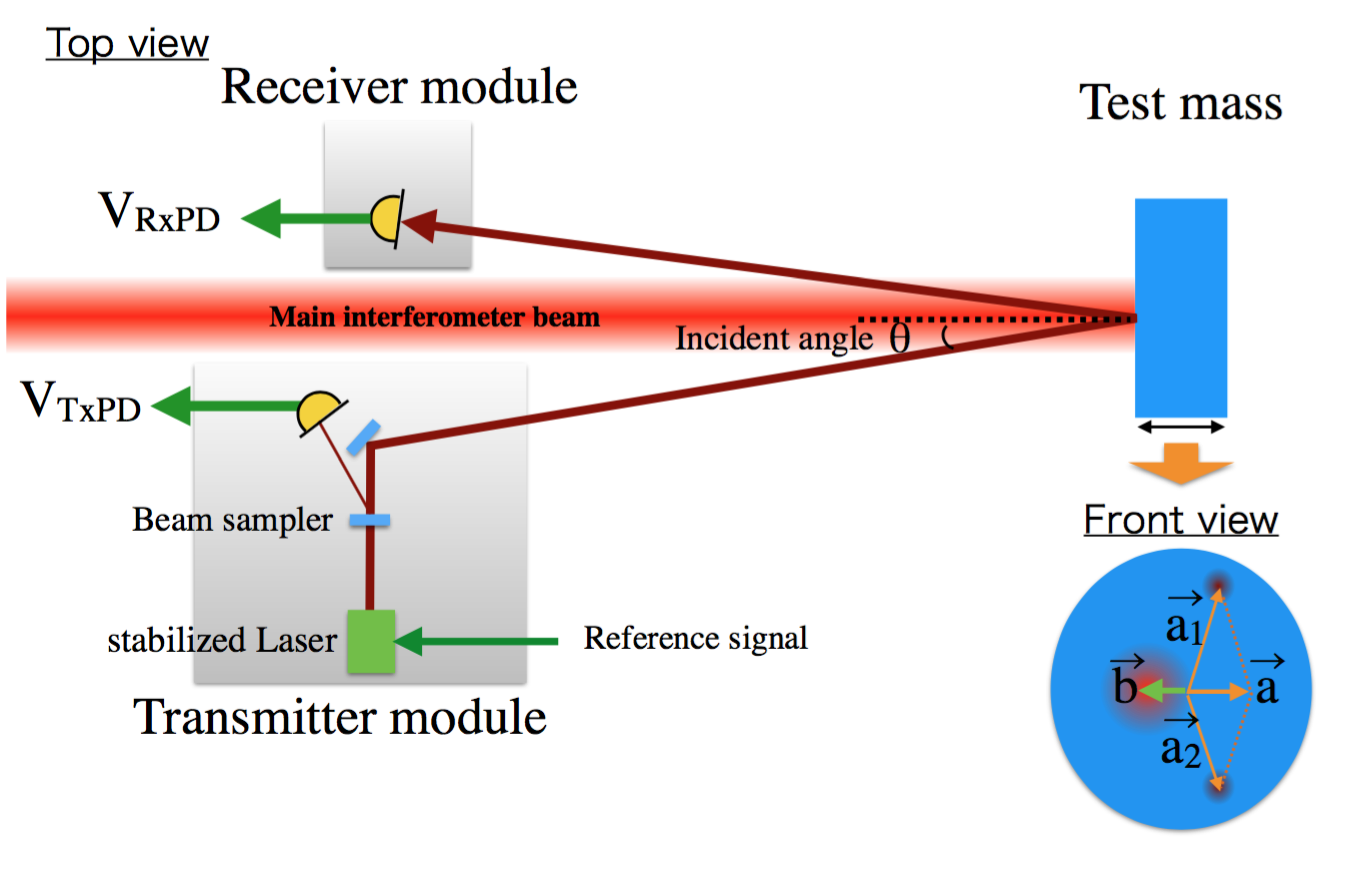
\includegraphics[width=12cm]{Pcal.eps}
\caption{Schematic view of photon calibrator. We place the stabilized laser on the transmitter module. The injected signal at the test masses is monitored by using the responces of photo detector power between the transmitter module, $V_{TxPD}$ and  receiver module, $V_{RxPD}$.  The geometrical factor is characterized by the position vector of the main beam, $\vec{a}=\vec{a_1}+\vec{a_2}$, and photon calibrator beams, $\vec{b}$.}
\label{fig:Pcal}
\end{center}
\end{figure}

\begin{table}
\begin{center}
\caption{Specification summary of LIGO, Virgo and KAGRA photon calibrator\label{pcal}}
\footnotesize
\begin{tabular}{cccc}
\hline
& KAGRA& advanced LIGO& advanced Virgo \\
\hline
Mirror material & Sapphire & Silica & Silica \\
 Mirror mass & 22.8 kg & 40 kg & 40 kg \\
  Mirror diameter & 220 mm & 340 mm & 350 mm \\
    Mirror thickness & 150 mm & 200 mm & 200 mm \\
 Distance of Pcal from ETM & 36 m & 8 m & 1.5 m \\
  Pcal laser power & 20 W & 2W & 3 W \\
  Laser frequency & 1047 nm & 1047 nm &1047 nm\\
  Incident angle& 0.72 deg & 8.75 deg &30 deg \\
  \hline
\end{tabular}
\end{center}
\end{table}

\section{Gravity field calibrator} \label{sec:Gcal}
To solve the uncertainty problem of the absolute calibration, we propose the gravity field calibrator. The gravity field calibrator generate the gravity field at the end of test mass by rotating the multipole masses. The rotor placed in the vacuum chamber for isolating the acoustic noise. To monitor the frequency, we mount the 10-bit encoder. We monitor the frequency using 16 bit ADC system.
We calculated the displacement by changing dynamic gravity field of multipole moment with with N masses.
The assumed model is the suspended test masses for the interferometer and disk with multipole mass as shown in Fig ~\ref{fig:dim}.
We put the masses $m$ at the positions of the radius $r$. The distance between the center of mass of mirror and disk is assumed $d$.
We rotate the disk at the angular frequency of $\omega_{rot}=2\pi f_{rot}$.

\begin{figure}
\begin{center}
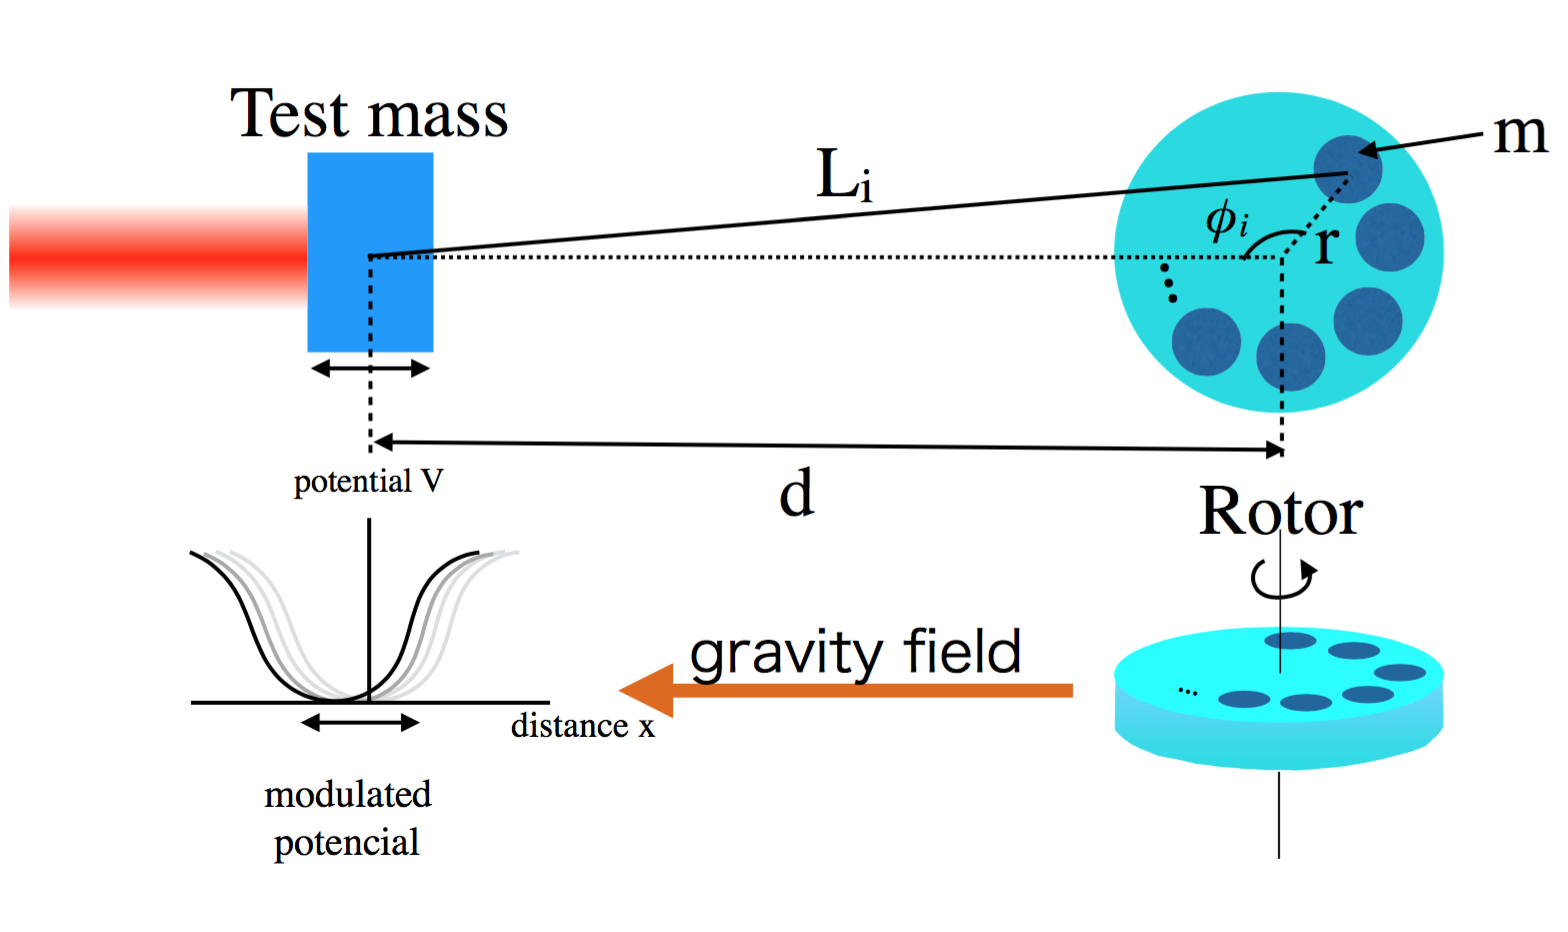
\includegraphics[width=12cm]{dim.eps}
\caption{Schematic view of gravity field calibrator. We placed the rotor at the displacement of $d$ away from test masses. Multipole mass generate the gravitational potential at the test mass position.}
\label{fig:dim}
\end{center}
\end{figure}

Distance between i-th mass and center of test mass is 
\begin{equation}
L_i=d \sqrt{1+\left( \frac{r}{d} \right)^2 -2\left( \frac{r}{d} \right) \cos{\phi_i} },
\end{equation}
where the angle of i-th mass is assumed as $\phi_i=\omega_{rot} t + 2\pi i/N$.
The gravity potential at the center of test mass can be described as
\begin{eqnarray}
V &=& \Sigma^N_{i=0} V_i \\
&=&-\frac{GMm}{d} \Sigma^N_{i=0} \Sigma^{\infty}_{n=0} \left( \frac{r}{d} \right)^n P_n\left(\cos{\left(\omega_{rot} t +\frac{2 \pi i}{N}\right)}\right),
\end{eqnarray}
where $P_n$ is Legendre polynomial. The equation of motion of test mass is 
\begin{equation}
Ma=\left| \frac{\partial V}{\partial{d}} \right| =\frac{GMm}{d^2}\Sigma^N_{i=0} \Sigma^{\infty}_{n=0}(n+1) \left( \frac{r}{d} \right)^n P_n\left(\cos{\left(\omega_{rot} t +\frac{2 \pi i}{N}\right)}\right),
\end{equation}
where $a$ is acceleration of test mass. We place the quadrupole and hexapole masses in same rotor as shown in Fig.~\ref{fig:hex}. We put the hole between each mass. The hole can increase the gravity gradient twice at the test masses effectively. Therefore, we can describe the equation of motion as 
\begin{equation}
Ma=\left| \frac{\partial V}{\partial{d}} \right| =\frac{2GMm}{d^2}\Sigma^N_{i=0} \Sigma^{\infty}_{n=0}(n+1) \left( \frac{r}{d} \right)^n P_n\left(\cos{\left(\omega_{rot} t +\frac{2 \pi i}{N}\right)}\right),
\end{equation}
We will calculate the displacement of quadrupole and hexapole in the section ~\ref{Quad} 

\begin{figure}
\begin{center}
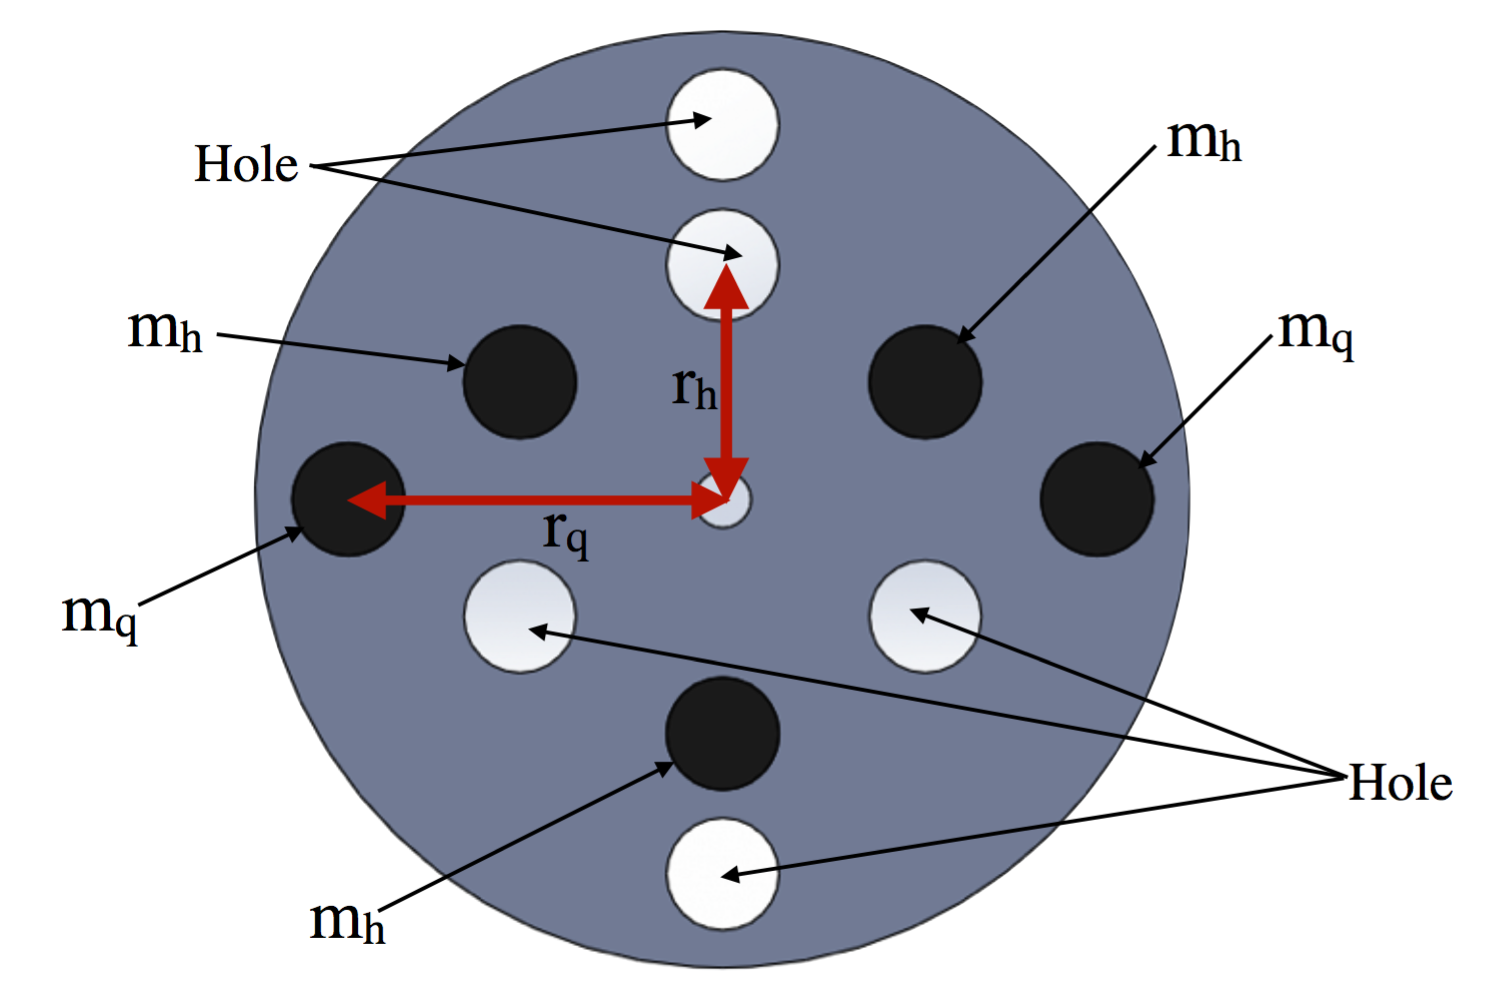
\includegraphics[width=12cm]{Hexapole.eps}
\caption{Configuration of the rotor with quadrupole and haxapole mass distribution.$m_q$ and $m_h$ are mass of quadrupole and hexapole. $r_q$ and $r_h$ are radius of quadrupole and hexapole.}
\label{fig:hex}
\end{center}
\end{figure}

\subsection{Displacement of test mass(Quadrupole)} \label{Quad}
We calculate the displacement of the quadrupole mass distribution corresponding to $N=2$.
The mass and radius of quadrupole are assumed as $m_q$ and $r_q$. 
The equation of motion of test mass is described as
\begin{equation}
Ma=\frac{2GMm_q}{d^2}\Sigma^{\infty}_{n=0}(n+1) \left( \frac{r_q}{d} \right)^n \left( P_n\left(\cos{\left(\omega_{rot} t \right)}\right) + P_n\left(\cos{\left(\omega_{rot} t +\pi \right)}\right) \right).
\end{equation} 
If we assume $r \ll d$, the displacement of the time-dependent lower harmonics can be written by 
\begin{equation}
x=\Sigma_{i=1}^{\infty}x_{n\mathrm{f}}\cos(n\omega_{rot} t)\sim x_{2\mathrm{f}}\cos(2\omega_{rot} t)=x_{2f}\cos{\omega t},
\end{equation}
where amplitude of 2-f rotation is
\begin{equation}
x_{2\mathrm{f}}=9\frac{GMm_{q}r_{q}^2}{d^4}s(\omega). \label{2f}
\end{equation}

\subsection{Displacement of test mass(Haxapole)} \label{Hexa}
We calculate the displacement of the hexapole mass distribution, which corresponds to $N=3$.
The mass and radius of hexapole are assumed as $m_h$ and $r_h$. 
The equation of motion of test mass is described as
\begin{eqnarray}
Ma = \frac{2GMm_h}{d^2}\Sigma^{\infty}_{n=0}(n+1) \left( \frac{r_h}{d} \right)^n \\
\times \left( P_n\left(\cos{\left(\omega_{rot} t \right)}\right) + P_n\left(\cos{\left(\omega_{rot} t+\frac{2\pi}{3} \right)} \right) + P_n\left(\cos{\left(\omega_{rot} t \frac{4\pi}{3} \right) }\right) \right).
\end{eqnarray} 
If we assume $r \ll d$, the displacement of the time-dependent lower harmonics can be written by 
\begin{equation}
x=\Sigma_{i=1}^{\infty}x_{n\mathrm{f}}\cos(n\omega_{rot} t)\sim  x_{3\mathrm{f}}\cos(3\omega_{rot} t)=x_{3f}\cos{\omega t},
\end{equation}
where amplitude of 3-f is
\begin{equation}
 x_{3\mathrm{f}}=15\frac{GMm_{h}r_{h}^3}{d^5}s(\omega). \label{3f}
\end{equation}

\section{Absolute power calibration by using Gcal and Pcal}
In this section, we will discuss about absolute laser power calibration using interferometer. 
Figure~\ref{fig:IFO} shows the configuration of absolute laser power calibration by using the combination of photon calibrator and gravity field calibrator.
First, we modulate the mirror position using gravity field calibrator. We can measure the signal of $x_{2f}$ and $x_{3f}$ in the response o interferometer. Second, we send the interferometer signal to the excitation port of photon calibrator as a reference of feedback control. The photon calibrator cancel the displacement by gravity field calibrator. Third, we measure the response of the detector of transmitter module and receiver module, whose unit is volt. The output signal of transmitter module, $V_{TxPD}$ and receiver module, $V_{RxPD}$ corresponding to displacement from gravity ffield should be modulated. By using Eq~(\ref{pcal}),(\ref{2f}), and (\ref{3f}), the modulated powers are
\begin{eqnarray}
 P_{2f}=18 \frac{Gcm_{q}Mr_{q}^2}{d^4cos\theta}\frac{1}{1+\frac{M}{I}\vec{a}\cdot \vec{b}} \label{2f} \\
 P_{3f}= 30\frac{Gcm_{h}Mr_{h}^3}{d^5cos\theta}\frac{1}{1+\frac{M}{I}\vec{a}\cdot \vec{b}} \label{3f}
\end{eqnarray}
Fourth, we demodulate the signal of transmitter module and receiver module using the encoder signal of gravity field calibrator.
The demodulated signals are 
\begin{eqnarray}
V_{2f}^{T}=\rho_{T}P_{2f} \\
V_{2f}^{R}=\rho_{R}P_{2f} \\
V_{3f}^{T}=\rho_{T}P_{3f} \\
V_{3f}^{R}=\rho_{R}P_{3f} 
\end{eqnarray} 
Therefore, we can estimate the distance using measured datas. 
\begin{equation}
d=\frac{5}{3} \frac{V_{2f}^T}{V_{3f}^T}\frac{m_{h}}{m_{q}}\frac{r_{h}^{3}}{r_{q}^{2}}=\frac{5}{3} \frac{V_{2f}^R}{V_{3f}^R}\frac{m_{h}}{m_{q}}\frac{r_{h}^{3}}{r_{q}^{2}} \label{d}
\end{equation}
Using Eq (\ref{d}),(\ref{2f}) and (\ref{3f}), we can calibrate the absolute leaser power.
Finally, we insert the equatin (\ref{2f}) to the equation (\ref{pcal}):
\begin{eqnarray}
x&=&\frac{P(\omega) \cos{\theta}}{2c} s(\omega)\left(1+\frac{M}{I}\vec{a} \cdot \vec{b} \right) \\
 &=&9\frac{P(\omega)}{P_{2f}}\frac{Gm_q M r_q^2}{d^4}s(\omega) , \\
 &=&\frac{729}{625} \frac{G m^5_q r_{q}^{10}}{m^4_h r_h^{12} \omega^2} \frac{{V_{3f}^{R}}^4}{{V_{2f}^{R}}^5}V^R(\omega) .\\
 &=&\frac{729}{625} \frac{G m^5_q r_{q}^{10}}{m^4_h r_h^{12} \omega^2} \frac{{V_{3f}^{R}}^4}{{V_{2f}^{R}}^5}V^R_0 \cos{\omega t} .\\ 
\end{eqnarray}

\begin{figure}
\begin{center}
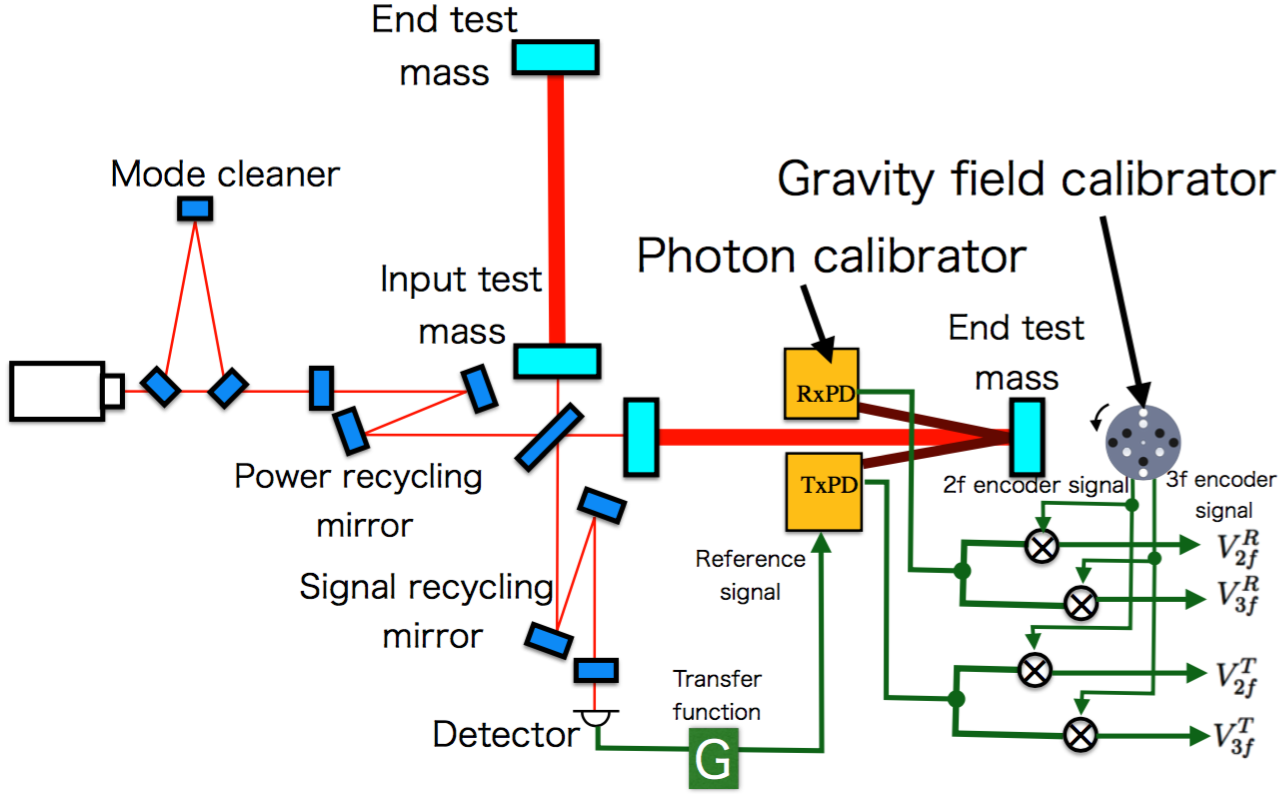
\includegraphics[width=12cm]{IFO.eps}
\caption{Test setup of the calibration of the laser power by rotating gravity field calibrator.}
\label{fig:IFO}
\end{center}
\end{figure}

\section{Estimation of uncertainty}
We estimate the uncertainty of displacement by assuming KAGRA. The assumed parameters are listed in Table~\ref{sus}. The optimization of the parameter of radius is important. To reduce the uncertainty of displacement, we put the quadrupole at the outer side and hexapole at the inner side.
\begin{table}
\begin{center}
\caption{\label{sus}The assumed parameters.}
\footnotesize
\begin{tabular}{cccc}
\hline
&&Value&Relative uncertainty \\
\hline
$G$& Gravity constant&6.6742&0.015 \%\\
$c$& speed of light[m/sec]&2.99792458e8&\\
$\theta$& Incident andgle&0.7[deg]& 0.07\%\\
$M$& Mass of test mass[kg]&23 & 0.02 \%\\
$m_q$&Mass of quadrupole[kg]&4.485 & 0.004 \%\\
$m_h$&Mass of hexapole[kg]& 4.485 &0.004\%\\
$r_q$&Radius of quadrupole[m]&0.200 & 0.025 \%\\
$r_h$&Radius of hexapole[m]& 0.125 & 0.04\%\\
$1+\frac{I}{M}\vec{a}\cdot \vec{b}$& Geometrical factor & 1&0.3 \% \\
\hline
\end{tabular}\\
\end{center}
\end{table}

\subsection{Systematic error of the higher order term}
If we consider the precision less than 1 \%, we need to consider the higher order of Legendre polynomial. This is because that higher order also has 2-f and 3-f components. These factor is mitigated by the factor of $(r/g)^n$, where $n$ is order of Legendre polynomial. Table XXX shows the higher order term. To compare the higher order effect by changing distance, we simulate the $x_{2f}$ and $x_{3f}$ using the FET method as shown in Fig~\ref{fig:ratio}. 

\begin{table}
\begin{center}
\caption{N=2,$\omega=n\omega_{rot}$ \label{pcal}}
\footnotesize
\begin{tabular}{ccccccc}
\hline
modulation& n=1 & n=2& n=3 &n=4&n=5&n=6 \\
\hline
1f&0&0&0&0&0&0 \\
2f&0&$9 \frac{Gmr^2}{d^4\omega^2}$&0&$\frac{25}{4} \frac{Gmr^4}{d^6\omega^2}$&0&$\frac{33075}{128} \frac{Gmr^6}{d^8\omega^2}$  \\
3f&0&0&0&0&0&0\\
4f&0&0&0&$\frac{175}{16} \frac{Gmr^4}{d^6\omega^2}$&0& $\frac{3675}{64} \frac{Gmr^6}{d^8\omega^2}$ \\
5f&0&0&0&0&0&0 \\
6f&0&0&0&0&0&$\frac{1617}{128} \frac{Gmr^6}{d^8\omega^2}$  \\
\hline
\end{tabular}
\end{center}
\end{table}

\begin{table}
\begin{center}
\caption{N=3,$\omega=n\omega_{rot}$ \label{pcal}}
\footnotesize
\begin{tabular}{ccccccc}
\hline
modulation& n=1 & n=2& n=3 &n=4&n=5&n=6 \\
\hline
1f&0&0&0&0&0&0 \\
2f&0&0&0&0&0&0  \\
3f&0&0&$15\frac{Gmr^3}{d^5\omega^2}$&0&$\frac{1449}{32}\frac{Gmr^5}{d^7\omega^2}$&0\\
4f&0&0&0&0&0&0 \\
5f&0&0&0&0&0&0 \\
6f&0&0&0&0&0&$\frac{4851}{256} \frac{Gmr^6}{d^8\omega^2}$  \\
\hline
\end{tabular}
\end{center}
\end{table}

\begin{figure}
\begin{center}
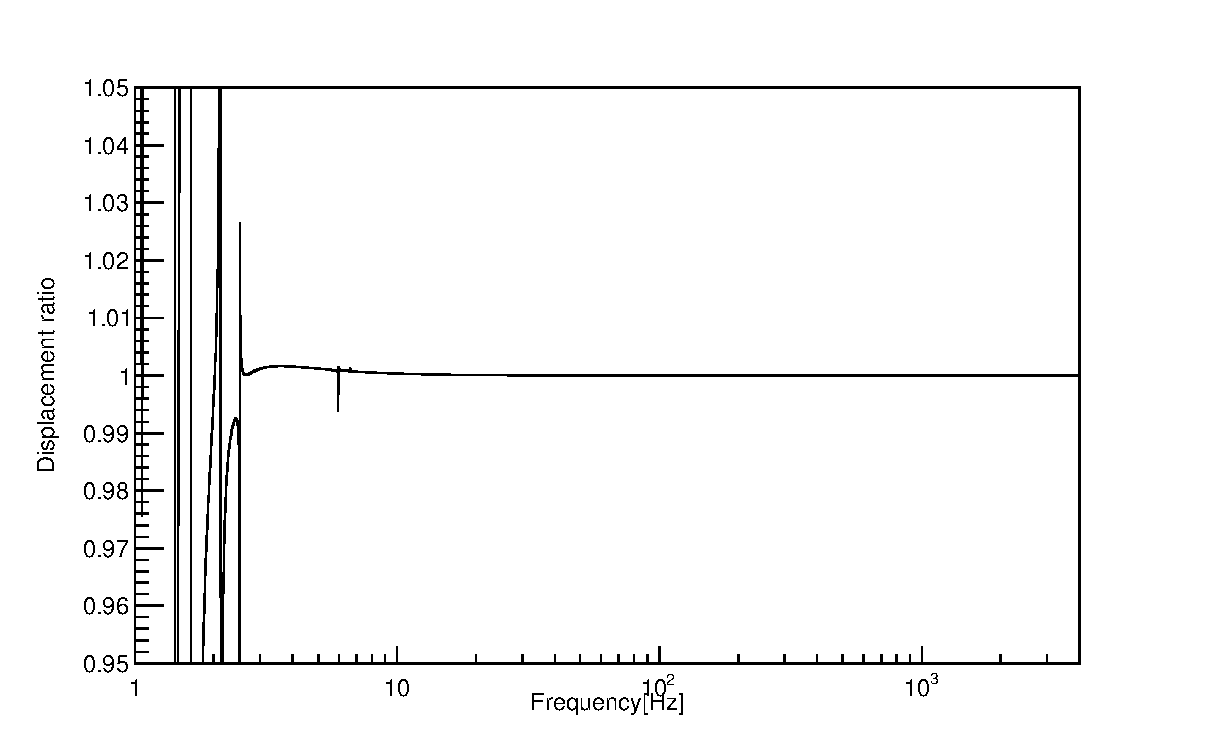
\includegraphics[width=12cm]{dx_Gcal_ratio.eps}
\caption{}
\label{fig:ratio}
\end{center}
\end{figure}
\subsection{Systematic error of the transfer function}
\begin{figure}
\begin{center}
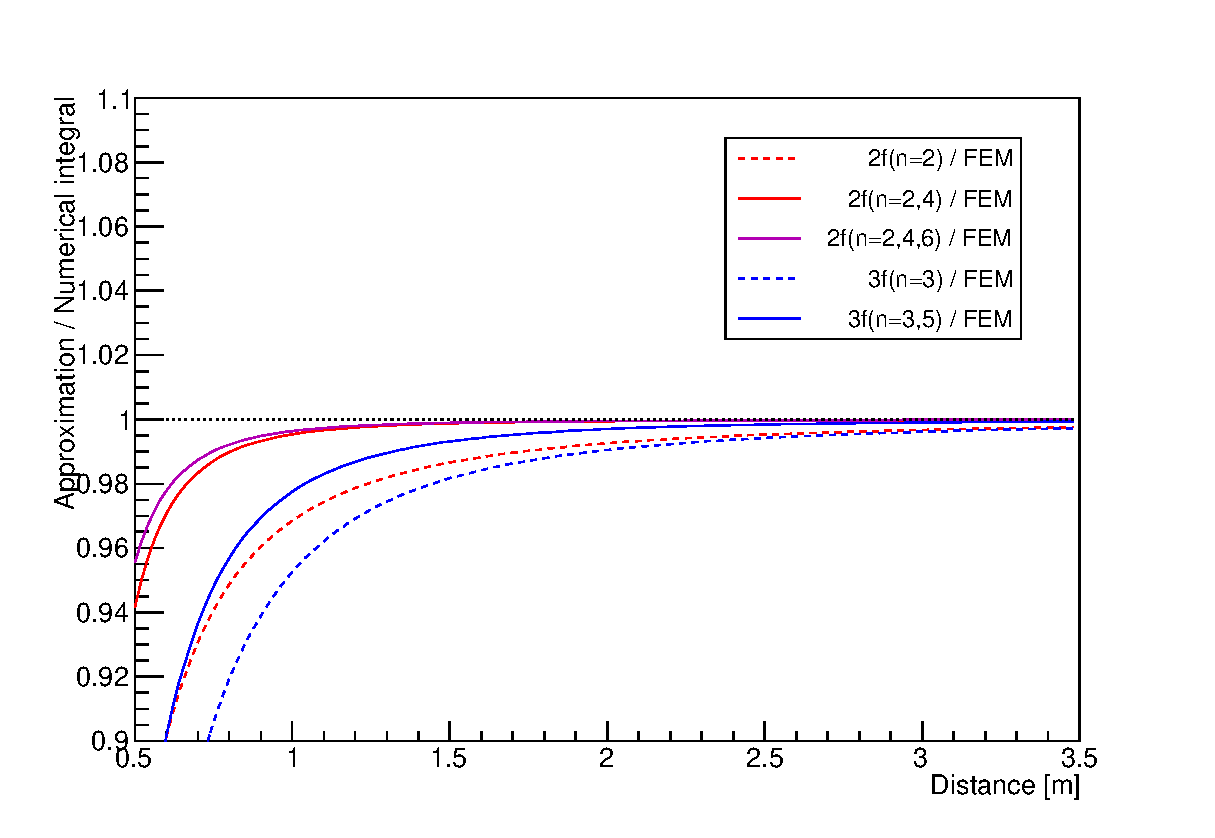
\includegraphics[width=12cm]{dvsx_ratio.eps}
\caption{}
\label{fig:ratio}
\end{center}
\end{figure}

We need to pay attention to the modulation effect of the intermediate mass because the gravity field act all the mass. We calculate the responses of the each masses using transfer function of KAGRA as shown in Fig XXX. We can neglect the intermediate mass effect and regard as free mass motion larger than XXXXX Hz. 

\subsection{Uncertainty of displacement and  laser power}
 The estimated displacements of 2f and 3f are described as
\begin{eqnarray}
x^{rms}_{2f}&=&1.178 \times 10^{-16}\mathrm{[m]} \times \left( \frac{G}{6.6742 \times 10^{-11} \mathrm{[m^3kg^{-1}sec^{-2}]}} \right) \times \left( \frac{m_q}{4.485 \mathrm{[kg]}} \right) \times \left( \frac{r_q}{0.200 \mathrm{[m]}} \right)^2 \\
 &&\times \left( \frac{2\mathrm{[m]}}{d} \right)^4 \times \left( \frac{2\pi(2\times 16)\mathrm{[Hz]}}{\omega} \right)^2\\
x^{rms}_{3f}&=&2.130 \times 10^{-18}\mathrm{[m]} \times \left( \frac{G}{6.6742 \times 10^{-11} \mathrm{[m^3kg^{-1}sec^{-2}]}} \right) \times \left( \frac{m_h}{4.485 \mathrm{[kg]}} \right) \times \left( \frac{r_h}{0.125 \mathrm{[m]}} \right)^3 \\
 &&\times \left( \frac{2\mathrm{[m]}}{d} \right)^5 \times \left( \frac{2\pi(3\times 16)\mathrm{[Hz]}}{\omega} \right)^2,
\end{eqnarray}
where the estimated value should correspond to the laser power for cancelation. 
The estimated powers are
\begin{eqnarray}
P_{2f}&=&0.09288 ~\mathrm{[W]}\times \left( \frac{G}{6.6742 \times 10^{-11} \mathrm{[m^3kg^{-1}sec^{-2}]}} \right)\times \left( \frac{c}{2.99792458 \times 10^{8} \mathrm{[m sec^{-1}]}} \right)\\
&& \times \left( \frac{m_q}{4.485 \mathrm{[kg]}} \right) \times \left( \frac{r_q}{0.200 \mathrm{[m]}} \right)^2 \times \left( \frac{2\mathrm{[m]}}{d} \right)^4 \times \left( \frac{1}{\cos{\theta}} \right) \times \left( \frac{1}{1+\frac{M}{I}\vec{a}\cdot \vec{b}} \right)^2\\
P_{3f}&=&0.003779~\mathrm{[W]} \times \left( \frac{G}{6.6742 \times 10^{-11} \mathrm{[m^3kg^{-1}sec^{-2}]}} \right)\times \left( \frac{c}{2.99792458 \times 10^{8} \mathrm{[m sec^{-1}]}} \right)\\
&& \times \left( \frac{m_h}{4.485 \mathrm{[kg]}} \right) \times \left( \frac{r_h}{0.125 \mathrm{[m]}} \right)^3 \times \left( \frac{2\mathrm{[m]}}{d} \right)^5 \times \left( \frac{1}{\cos{\theta}} \right) \times \left( \frac{1}{1+\frac{M}{I}\vec{a}\cdot \vec{b}} \right)^2.
\end{eqnarray}
The ratio of the powers corresponds to $V^T_{2f}/V^{T}_{3f}$ and is proportional to the distance. The estimated $V^T_{2f}/V^{T}_{3f}$ by changing distance are shown in Fig.~\ref{fig:dvsVV}.

\begin{figure}
\begin{center}
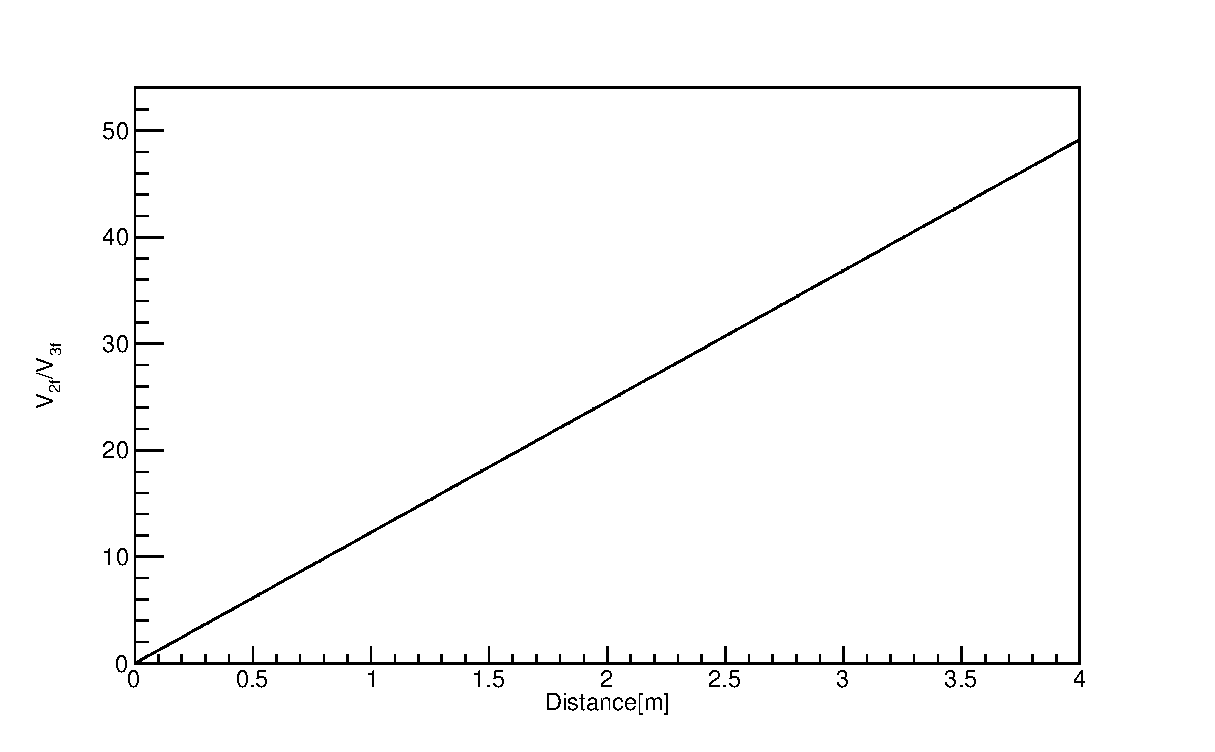
\includegraphics[width=12cm]{dvsVV.eps}
\caption{}
\label{fig:dvsVV}
\end{center}
\end{figure}
The uncertainty of the quadrupole and hexapole masses are limited by the accuracy of electronic balance. In this case, we use the weight made of Tungsten. The density of Tungsten is $19.25~\mathrm{g/cm^3}$. The diameter and thickness of mass are 0.06m and 0.08~m, respectively. Therefore, mass of the rotor mass is 4.485~kg. To measure this mass, we assumed that we use an electronic balance whose catalog number and accuracy are CG-6000 and 0.2~g. Therefore, the relative uncertainty of the mass of rotor mass is 0.04~\%.

 To make the rotor disc, we use the NC milling machine. The typical accuracy is less than 0.02 mm. For the measuring of the shape, we employ the three-dimension coordinate measuring machine (CMM). The precision of CMM is $2~\mathrm{\mu m}$. We measure the precision of rotor and estimate the uncertainty. The estimated relative uncertainty of  displacement is written as
\begin{eqnarray}
\left( \frac{\delta x}{x} \right)^2 &\sim& \left( \frac{\delta G}{G} \right)^2 +\left( \frac{\delta V^R_0}{V^R_0} \right)^2+4\left( \frac{\delta \omega}{\omega} \right)^2+ 25\left( \frac{\delta m_q}{m_q} \right)^2 +16\left( \frac{\delta m_h}{m_h} \right)^2 \\
&+&25\left( \frac{\delta V^R_{f2}}{V^R_{f2}} \right)^2+16\left( \frac{\delta V^R_{f3}}{V^R_{f3}} \right)^2+ 100\left( \frac{\delta r_q}{r_q} \right)^2 +144\left( \frac{\delta r_h}{r_h} \right)^2.
\end{eqnarray}
As you can see, the contribution of the radius uncertainty is amplified by the factor. To reduce the noise of displacement, we need to reduce the uncertainty of the mass positions.
The uncertainty of the $V^R_{2f}$,$V^R_{3f}$, $V^R_{0}$ are the measured value. It implies that we can reduce the uncertainty with long time integration time due to the statistics. Each the uncertainty is listed in Table.~\ref{sus}. The estimated uncertainty is XXX \%.
We can also estimate the laser power by using the following equations:
\begin{eqnarray}
\left( \frac{\delta P_{2f}}{P_{2f}} \right)^2 &\sim& \left( \frac{\delta G}{G} \right)^2 +\left( \frac{\delta c}{c} \right)^2+ \left( \frac{\delta M}{M} \right)^2+25\left( \frac{\delta m_q}{m_q} \right)^2+16\left( \frac{\delta m_h}{m_h} \right)^2 +100\left( \frac{\delta r_q}{r_q} \right)^2+144\left( \frac{\delta r_h}{r_h} \right)^2 \\
&+&16\left( \frac{\delta V^R_{f2}}{V^R_{f2}} \right)^2+16\left( \frac{\delta V^R_{f3}}{V^R_{f3}} \right)^2+16\left( \frac{\delta d}{d} \right)^2+\left( \frac{\delta (\cos{\theta})}{\cos{\theta}} \right)^2+ \left( \frac{\delta\left( \frac{1}{1+\frac{M}{I}\vec{a}\cdot \vec{b}} \right)}{\left( \frac{1}{1+\frac{M}{I}\vec{a}\cdot \vec{b}} \right)} \right)^2 \\
\left( \frac{\delta P_{3f}}{P_{3f}} \right)^2 &\sim& \left( \frac{\delta G}{G} \right)^2 +\left( \frac{\delta c}{c} \right)^2+ \left( \frac{\delta M}{M} \right)^2+25\left( \frac{\delta m_q}{m_q} \right)^2+16\left( \frac{\delta m_h}{m_h} \right)^2 +100\left( \frac{\delta r_q}{r_q} \right)^2+144\left( \frac{\delta r_h}{r_h} \right)^2 \\
&+&16\left( \frac{\delta V^R_{f2}}{V^R_{f2}} \right)^2+16\left( \frac{\delta V^R_{f3}}{V^R_{f3}} \right)^2+16\left( \frac{\delta d}{d} \right)^2+\left( \frac{\delta (\cos{\theta})}{\cos{\theta}} \right)^2+ \left( \frac{\delta\left( \frac{1}{1+\frac{M}{I}\vec{a}\cdot \vec{b}} \right)}{\left( \frac{1}{1+\frac{M}{I}\vec{a}\cdot \vec{b}} \right)} \right)^2 \\
\end{eqnarray}

The estimated relative uncertainties of the powers are XXXXX. One of the largest uncertainty is the geometrical factor of the Pcal laser. The geometrical factor uncertainty is assumed 0.3 \%, which is same number of LIGO. The estimated total uncertainties are XXXXX and XXXXX. However, KAGRA employ the beam position monitoring system. It expected to reduce the its uncertainty less than 0.3\%. 


\section{Conclusion}
Photon calibrator is one of the powerful calibrators in LIGO, Virgo and KAGRA. It can calibrate the response of IFO and its uncertainty is essential for estimation of gravitational wave source. In particular, the distance of the source is strongly depend on the absolute laser power of the photon calibrator. In previous study, the Gold standard, which response is calibrated by the laser power standard of NIST, is used for the absolute laser power calibration of the photon calibrator. However, current limit of the absolute laser power between each country is about XXX \%. It is directly propagate to the uncertainty of absolute displacement of gravitational wave detector.

To solve the problem, we proposed the combination method of photon calibrator and gravity field calibrator. Gravity field calibrator can modulate the mirror using gravity gradient. By canceling the displacement of the test mass using the photon calibrator, we can calibrate the absolute laser power and displacement of the photon calibrator with accuracy of 0.XXX \%.

This method has an advantage of a direct comparison of the amplitude of injected power and gravity field. In previous study, we need to consider the uncertainty of the optical efficiency through the window and mirrors. This is because we put the working standard at the outside of the chamber. However, the method of gravity field can compare the displacement directly. By using this method, we can calibrate the uncertainty of optical efficiency and absolute power of the laser. When we compare the laser power between each institute, we need to bring the working standard. However, we can try the absolute calibration using this method. As we mention about a few percent of the absolute uncertainty of laser in each country. The estimated uncertainty of the power of this method is less than 1 \%. It imply that we can make a new power standard using interferometer.
%%%%%%%%%%%%%%%%%%%%%%%%%%%%%%%%%%%%%%%%%%%%%%%%%%%%%%%%%%%%%
\acknowledgments     %>>>> equivalent to \section*{ACKNOWLEDGMENTS}       
 
We thank Rechard Savage, Darkhan Tuyrnbayev for diskussion of the photon calibrator. We would like to express our gratitude to Prof.Takaaki Kajita and Prof.Henry Wong. We would like to thank the KEK Cryogenics Science Center for the support. YI was supported by Academia Sinica under Grants No. CDA-105-M06 in Taiwan. This work was supported by JSPS KAKENHI Grant Numbers XXXXXX and XXXXXX, and by the JSPS Core-to-Core Program.

%%%%%%%%%%%%%%%%%%%%%%%%%%%%%%%%%%%%%%%%%%%%%%%%%%%%%%%%%%%%%
%%%%% References %%%%%

\bibliography{report}   %>>>> bibliography data in report.bib
\bibliographystyle{spiebib}   %>>>> makes bibtex use spiebib.bst

\end{document} 
